% ============================================================
% ICAIS 2026 Track 2: 少年科学家 | 4-Page Compact
% 频谱免疫：AI科学家物理量导出的频域可靠性审计框架
% 终稿 v9 - 与英文版完全对应（疏松版）
% ============================================================
\documentclass[9pt,twocolumn]{article}

% ============ 基础设置 ============
\usepackage[UTF8]{ctex}
\usepackage[english]{babel}
\usepackage{amsmath,amssymb,amsfonts}
\usepackage{amsthm}
\usepackage{booktabs}
\usepackage{multirow}
\usepackage[font=scriptsize,labelfont=bf,skip=0pt]{caption}
\usepackage[hidelinks,colorlinks=true,linkcolor=black,citecolor=black,urlcolor=black]{hyperref}
\usepackage[margin=1.3cm,columnsep=0.45cm,top=1.6cm,bottom=1.1cm]{geometry}
\usepackage{setspace}
\usepackage{fancyhdr}
\usepackage{float}
\usepackage{enumitem}
\usepackage{titlesec}
\usepackage{array}
\usepackage{xcolor}
\usepackage{mathtools}
\usepackage{bm}
\usepackage{graphicx}
\usepackage{algorithm}
\usepackage{algpseudocode}

% ============ 定理环境 ============
\newtheorem{proposition}{命题}
\newtheorem{theorem}[proposition]{定理}
\theoremstyle{remark}
\newtheorem{remark}[proposition]{注记}
\theoremstyle{definition}
\newtheorem{definition}[proposition]{定义}

% ============ 页面设置（疏松版） ============
\setlength{\parindent}{0.5em}
\setlength{\parskip}{0.5pt}
\renewcommand{\baselinestretch}{0.78}          % 从0.68放宽到0.78
\setlength{\abovecaptionskip}{1.5pt}
\setlength{\belowcaptionskip}{0.5pt}
\setlength{\floatsep}{3pt}
\setlength{\textfloatsep}{3pt}
\setlength{\intextsep}{2pt}
\setlength{\abovedisplayskip}{1.5pt}
\setlength{\belowdisplayskip}{1.5pt}
\setlength{\abovedisplayshortskip}{1pt}
\setlength{\belowdisplayshortskip}{1pt}

\pagestyle{fancy}
\fancyhf{}
\fancyhead[L]{\scriptsize\itshape ICAIS 2026 Track 2: 少年科学家}
\fancyhead[R]{\scriptsize\thepage}
\renewcommand{\headrulewidth}{0.2pt}
\setlength{\headheight}{14pt}
\setlength{\headsep}{6pt}

\titleformat{\section}{\normalsize\bfseries}{}{0em}{}
\titlespacing{\section}{0pt}{2pt}{1pt}         % 节标题间距增加
\titleformat{\subsection}[runin]{\small\bfseries}{}{0em}{}
\titlespacing{\subsection}{0pt}{2pt}{2pt}      % 小节标题间距增加

\setlist{nosep,leftmargin=*,itemsep=0.5pt,topsep=0.5pt}

% ============ 自定义命令 ============
\newcommand{\pxrmse}{\sigma_{\text{px}}}
\newcommand{\physerr}{\epsilon_{\text{phys}}}
\newcommand{\nprf}{\text{NPRF}}
\newcommand{\snf}{S_n(f)}
\newcommand{\hsysf}{|H_{\text{sys}}(f)|^2}
\newcommand{\Hsqmean}{\overline{H^2}}
\newcommand{\Beff}{\mathcal{B}_{\text{eff}}}

% Compact algorithm setup
\makeatletter
\newcommand{\algorithmiccompact}{\renewcommand{\algorithmicrequire}{\textbf{输入：}}\renewcommand{\algorithmicensure}{\textbf{输出：}}}
\makeatother

\newcommand{\澔}{%
  \hbox{%
    \scalebox{0.75}[1]{氵}%
    \kern -0.3em%
    \scalebox{0.8}[1]{皓}%
  }%
}
\newcommand{\name}{%
  \mbox{%
    林%
    \kern -0.2em%
    \澔%
    \kern -0.02em%
    仁%
  }%
}

\begin{document}

\twocolumn[
\vspace{-4pt}
  \begin{center}
    {\Large\bfseries 频谱免疫：AI科学家物理量导出的频域可靠性审计框架}

    \vspace{3pt}

    {\small\bfseries 投稿至 ICAIS 2026 Track 2: 少年科学家}

    \vspace{4pt}

    {\small 杨御之\ \ \name \ $^{1}$}

    \vspace{1.5pt}

{\scriptsize $^{1}$ 南开中学，天津市，中国 \quad \texttt{mdrosslyning@gmail.com} \quad \texttt{daoming\_kan@163.com}}\quad {\scriptsize 指导教师：滕伟\ $^{1}$}

    \vspace{2pt}

    {\scriptsize\textbf{人类责任声明：}核心科学洞察、全部定理推导、实验设计与分析均由作者独立完成。AI工具仅用于Python代码语法调试与英文摘要润色。所有实验代码及数据完全可复现。}

    \vspace{3pt}
    \rule{\linewidth}{0.4pt}
  \end{center}
  \vspace{-4pt}
]

% ==================== 摘要 ====================
\section*{摘要}
\vspace{-0.5pt}
\begingroup
\scriptsize
\setlength{\parindent}{0.8em}
\setlength{\parskip}{0.8pt}

AI科学家系统的可靠性评估仍依赖像素级RMSE。其隐含假设——观测空间精度可代理物理空间准确度——本文称之为\textbf{像素幻觉}，在物理量导出场景中系统性失效。当误差功率谱密度在物理算子的共振频带内非平坦时，固定像素RMSE$=10^{-3}$条件下，白噪声与红噪声输入的物理误差比值达3.03倍。本文提出\textbf{频谱免疫框架}。其核心指标——归一化物理风险因子（NPRF）——以白噪声为基线，仅需AI输出残差的频谱估计和一次离线标定的算子频响，即可在推理阶段自动计算频谱健康度，无需物理真值。

实验揭示：（1）固定像素RMSE$=10^{-3}$下，白噪声产生153.5\%物理误差，而红噪声仅50.7\%；（2）幅度受控条件下，NPRF对物理误差的Spearman秩相关达0.968，与RMSE形成互补诊断；（3）早期预警案例显示两个模型具有\textit{完全相同的}像素RMSE（$0.00200$），但物理误差相差8.26倍（98.7\% vs.\ 815.3\%），NPRF正确标记（$0.113$ vs.\ $8.875$）；（4）标准MSE训练模型的残差频谱主要由信号频率结构而非训练噪声类型决定。消融实验确认60 Hz分量具有大效应量（$p=0.000042$，Cohen's $d=1.558$）；训练噪声类型效应在Bonferroni校正后\textit{不}具有统计显著性（$p=0.056$，功效$\approx0.35$），需更大样本；（5）标准Butterworth低通滤波在非稳态噪声下将NPRF恶化380.0\%；（6）后处理频谱重塑（五级陷波滤波）在不重新训练的情况下将NPRF降低49.8\%，物理误差降低31.0\%（$p=0.001953$）；（7）篮球抛体运动的初步真实世界实验获得NPRF$=0.177$（仅工作流演示；$N=53$不足以进行统计推断）。

\vspace{2pt}
\noindent\textbf{关键词：}AI-for-Science；频谱可靠性；NPRF；物理量导出；频谱免疫

\endgroup

\vspace{2pt}
\hrule
\vspace{2pt}

% ==================== 1. 引言 ====================
\section{引言}

\subsection{一个被忽视的问题}

2023至2024年，AI科学家系统在蛋白质结构预测（AlphaFold 3\cite{abramson2024}）、材料发现（GNoME\cite{merchant2023}）和全球天气预报（GraphCast\cite{lam2023}）等领域取得突破。它们的共同工作流是接收观测数据，经深度网络输出物理量。然而，一个根本性问题被系统性忽视：\textbf{AI科学家如何判断其物理量导出输出是否可靠？}

本文聚焦以下工作流的可靠性审计：

\begin{equation}
\label{eq:workflow}
\text{观测数据} \xrightarrow{\text{AI模型}} \hat{\mathbf{x}} \xrightarrow{\text{物理量导出算子}\ \mathcal{D}} \hat{a}
\end{equation}

其中$\hat{\mathbf{x}}$表示AI在观测空间的输出；$\mathcal{D}$是导出物理量的确定性算子（微分、反卷积、积分变换）。像素级RMSE评估第一阶段误差，而物理实验的可信度取决于第二阶段输出$\hat{a}$的误差。$\mathcal{D}$频响在特定频段的巨大增益可使两空间之间的映射被数量级放大。

在传统科学实践中，人类研究者通过重复实验、替代方法和理论预期进行交叉验证。当AI接管这些步骤后，可靠性评估被简化为像素级RMSE。这嵌入了一个未经检验的代理假设：观测空间精度可代理物理空间准确度。我们将这种未经质疑的接受命名为\textbf{像素幻觉}，并证明该假设系统性失效。

\textbf{为什么AI科学家特别需要此框架。}在自主实验室\cite{burger2020}中，AI科学家在闭环中生成假设、设计实验并解读结果；当评估器存在频谱盲区时，错误在无人察觉的情况下被写入知识库。深度网络对高频分量的拟合慢于低频分量\cite{xu2019,rahaman2019,tancik2020,ronen2019}；残差频谱天然非平坦。AlphaFold\cite{abramson2024}在数月内预测数亿个蛋白质结构；即使1\%的频谱盲区错误率也超过人类科学家一生所犯错误的总和。\textbf{频谱免疫因此是AI科学家元认知的核心组件。}

\textbf{范围界定。}本文不提出新的AI模型。相反，它解决的是：\textit{当AI模型输出物理量时，AI系统如何自行判断这些输出是否可信？}我们提供诊断工具（NPRF）、早期预警演示（实验2b）和补救方案（后处理重塑）。

\subsection{相关工作}

频谱偏置已有充分文献记载：深度网络先拟合低频分量\cite{rahaman2019,xu2019,tancik2020,ronen2019}。经典不确定性量化（贝叶斯方法\cite{kendall2017}、集成方法\cite{lakshminarayanan2017}）问的是"有多不确定？"而非"在物理上有多危险？"SG微分\cite{savitzky1964}放大高频噪声，但此前没有工作将算子频响与AI流程可靠性审计联系起来。我们填补了这一空白。

\subsection{物理真值沙盒（PGTS）}

我们构建了一个\textbf{物理真值沙盒（PGTS）}：匀加速轨迹（$a_{\text{ref}}=9.8$ m/s$^2$），加速度由21点三阶Savitzky-Golay滤波器\cite{savitzky1964}导出。SG滤波器的联合频响平方幅值$\hsysf$的共振峰位于$f_{\text{peak}}=51$ Hz；理论噪声放大因子为$\sqrt{\sum_{i=1}^{21} c_i^2}=13353.3$。像素残差RMSE为$10^{-3}$的追踪系统因此产生高达$13.35$ m/s$^2$的导出加速度RMSE，对应136.3\%的相对物理误差。白噪声实测153.5\%反映了有限信号长度下的SG边界效应。

\subsection{贡献}

两位作者贡献均等。（1）\textbf{诊断}（\S 2.1）：证明代理指标有效当且仅当误差PSD在算子有效通带内平坦。（2）\textbf{工具}（\S 2.2）：提出NPRF，无需物理真值。（3）\textbf{早期预警}（\S 3.3）：演示NPRF标记像素RMSE无法检测的8.26倍物理误差差异。（4）\textbf{补救}（\S 3.5）：验证后处理频谱重塑。

% ==================== 2. 频谱免疫理论 ====================
\section{频谱免疫理论}

\subsection{频谱对抗脆弱性}

考虑含噪轨迹$\hat{\mathbf{x}} = \mathbf{x} + \mathbf{n}$，噪声PSD为$\snf$。定义：
\begin{equation}
\label{eq:metrics}
\pxrmse = \sqrt{\mathbb{E}[(\hat{x}_i - x_i)^2]}, \quad \physerr = \frac{\text{RMSE}(\hat{a}, a_{\text{ref}})}{|a_{\text{ref}}|} \times 100\%.
\end{equation}

\begin{definition}[频谱对抗脆弱性]
设物理量由线性算子$\mathcal{D}$导出，联合传递函数为$H_{\text{sys}}(f)$。若两个噪声过程满足$\pxrmse^{(1)}=\pxrmse^{(2)}$但$\physerr^{(1)}\neq\physerr^{(2)}$，则该评估流程存在\textbf{频谱对抗脆弱性}。
\end{definition}

\begin{theorem}[代理指标有效性的充分条件]
\label{thm:sufficiency}
设$\mathcal{D}$为线性时不变系统，联合频响平方幅值为$\hsysf$。固定阈值$\theta \in (0,1)$。定义\textit{有效通带}：
\begin{equation}
\label{eq:band}
\Beff(\theta) = \bigl\{f \in [0, f_s/2] : \hsysf \geq \theta \cdot \max_{f'} \hsysf \bigr\},
\end{equation}
其中$|\Beff|$表示Lebesgue测度。若噪声PSD $\snf$满足：\textbf{(i) 有效支撑条件}——存在$\epsilon>0$使得$\int_{f \notin \Beff} \hsysf \,\snf \, df \leq \epsilon \int_{\Beff} \hsysf \,\snf \, df$且$\int_{f \notin \Beff} \snf \, df \leq \epsilon \int_{\Beff} \snf \, df$；\textbf{(ii) 近似平坦条件}——存在$S_0>0, \delta>0$使得$\sup_{f \in \Beff} |\snf - S_0|/S_0 \leq \delta$。则存在仅依赖于$\mathcal{D}$、$\theta$、$f_s$的$C(\theta)$使得
\begin{equation}
\label{eq:thm_bound}
\bigl|\physerr - C(\theta) \cdot \pxrmse \bigr| = O(\delta + \epsilon),
\end{equation}
其中$C(\theta) = \frac{1}{|a_{\text{ref}}|} \sqrt{\frac{\int_{\Beff} \hsysf \, df}{|\Beff|}}$。\textit{证明：}由Parseval恒等式\cite{brillinger2001}，$\operatorname{Var}[\hat{a}] = \int_{0}^{f_s/2} \hsysf \,\snf \, df$；结果由(i)--(ii)直接代入得出。
\end{theorem}

\begin{remark}[直观解释]
定理~\ref{thm:sufficiency}表明：\textbf{若噪声频谱在算子有效通带内近似平坦，则像素RMSE是物理误差的良好代理。}红噪声（低频集中）使RMSE\textit{高估}风险；共振带噪声使RMSE\textit{低估}风险。$\theta$典型取$10^{-3}$--$10^{-6}$。对于非线性系统，一阶Taylor局部线性化适用；该定理提供直觉而非紧界。实际应用中，NPRF（\S 2.2）作为操作指标，无需选择阈值。
\end{remark}

\subsection{归一化物理风险因子（NPRF）}

\begin{theorem}[物理误差的频谱变分原理]
\label{thm:variational}
在约束$\int \snf \, df = \pxrmse^2$且$\snf \geq 0$下，物理量方差的紧上界为$\pxrmse^2 \cdot \max_f \hsysf$。等号成立当且仅当$\snf$为集中于$\arg\max_f \hsysf$的Dirac-$\delta$分布。
\end{theorem}

\textbf{从通带到全频带归一化。}与定理~\ref{thm:sufficiency}的通带限制分析不同，NPRF使用$\hsysf$的全频带算术均值作为归一化基线。该选择解析可处理（无需选择阈值$\theta$）、直接可解释（白噪声$\Rightarrow$NPRF$=1$），且对有效通带可能多模态或定义不清的算子类型具有鲁棒性。

定义\textbf{归一化物理风险因子（NPRF）}：
\begin{equation}
\label{eq:nprf_def}
\nprf = \frac{\int_{0}^{f_s/2} \hsysf \,\snf \, df}{\pxrmse^2 \cdot \Hsqmean},
\end{equation}
其中$\Hsqmean = \frac{1}{f_s/2}\int_{0}^{f_s/2} \hsysf \, df$为$\hsysf$的算术均值。\textbf{NPRF等于$\hsysf$加权平均与$\hsysf$普通算术平均之比}，以白噪声为归一化基线。NPRF仅需残差的Welch谱估计\cite{welch1967}加上一次离线标定；\textbf{无需物理真值}。

\textbf{``归一化''的解读。}NPRF是\textit{相对于白噪声}归一化，而非相对于安全性。NPRF$=1.0$=白噪声基线，\textbf{不是}安全阈值（$\sigma_{\text{px}}=10^{-3}$的白噪声已产生153.5\%物理误差）。NPRF$<1.0$=给定相同像素RMSE下比白噪声更安全。绝对风险：
\begin{equation}
\label{eq:decomposition}
\sigma_a = \pxrmse \cdot \sqrt{\Hsqmean \cdot \nprf}.
\end{equation}

\textbf{部署工作流。}完整诊断流程总结于算法1。

\begin{algorithm}[htbp]
\scriptsize
\algorithmiccompact
\begin{algorithmic}[1]
\Require AI残差 $\mathbf{r}[n]$，已标定算子响应 $\hsysf$，采样率 $f_s$
\Ensure NPRF分数和风险标记
\State 估计PSD：$\snf \leftarrow \text{Welch}(\mathbf{r}, f_s)$ \Comment{$O(N\log N)$}
\State 计算像素RMSE：$\pxrmse \leftarrow \text{std}(\mathbf{r})$
\State 计算归一化：$\Hsqmean \leftarrow \frac{1}{f_s/2}\int \hsysf \, df$
\State 通过式~\eqref{eq:nprf_def}计算NPRF
\If{$\nprf > 2.0$}
    \State 标记：``高风险''；建议频谱免疫滤波器
\ElsIf{$\nprf > 1.5$}
    \State 标记：``中等风险''；建议检查
\Else
    \State 标记：``低风险（相对白噪声）''
\EndIf
\State \Return $\nprf$，标记
\end{algorithmic}
\caption{频谱免疫检查（部署就绪）}
\label{alg:nprf}
\end{algorithm}

\textbf{统计说明：}Bootstrap验证（$B=1000$）：$N=1000$时95\%置信区间$\approx\pm10\%$。Welch泄漏对集中频谱低估NPRF（零预测器：实测5.731 vs.\ 理论$\sim10^7$；加窗将谱线扩散至$\sim4$ Hz）。$N<200$：筛查；$N<100$：仅概念。\textbf{频谱疫苗} = \{NPRF诊断 + 频谱免疫滤波器\}。复杂度：$O(N\log N)$，$N=10^4$时$<1$ ms。

% ==================== 3. 实验验证 ====================
\section{实验验证}

\begingroup
\scriptsize
\textbf{可复现性：}所有实验使用固定随机种子。完整代码见附录。
\endgroup

\vspace{1pt}

\subsection{实验1：频谱对抗样本}

固定$\pxrmse = 0.001$。生成幂律噪声\cite{kasdin1995}，$\alpha=\{-2, 0, +2\}$，每组100次实现。

\begin{center}
    \scriptsize\setlength{\tabcolsep}{2.5pt}
    \begin{tabular}{lccc}
        \toprule
        \textbf{噪声（$\alpha$）} & $\bm{\physerr}$(\%) & $\nprf$ & \textbf{特征} \\
        \midrule
        红（$-$2） & $\mathbf{50.7_{\pm2.3}}$ & $0.126_{\pm0.013}$ & 被动安全 \\
        白（0）  & $153.5_{\pm16.6}$ & $0.981_{\pm0.077}$ & 基线 \\
        蓝（$+$2） & $71.2_{\pm10.6}$ & $0.195_{\pm0.010}$ & 主动安全 \\
        \bottomrule
    \end{tabular}
    \\[0.5pt]
    {\scriptsize \textbf{表1：}在相同像素RMSE（$10^{-3}$）下，白/红物理误差比值达3.03倍（$n=100$/组）。NPRF排序与物理误差排序一致。理论值136.3\%与实测153.5\%的偏差源于SG边界效应。蓝噪声将能量集中于共振带上方$|H_{SG}|^2$已衰减的区域，尽管高频含量高，物理误差反而低于白噪声。}
\end{center}

\textbf{核心发现：}NPRF正确排序相对风险。

\begin{figure}[htbp]
    \centering
    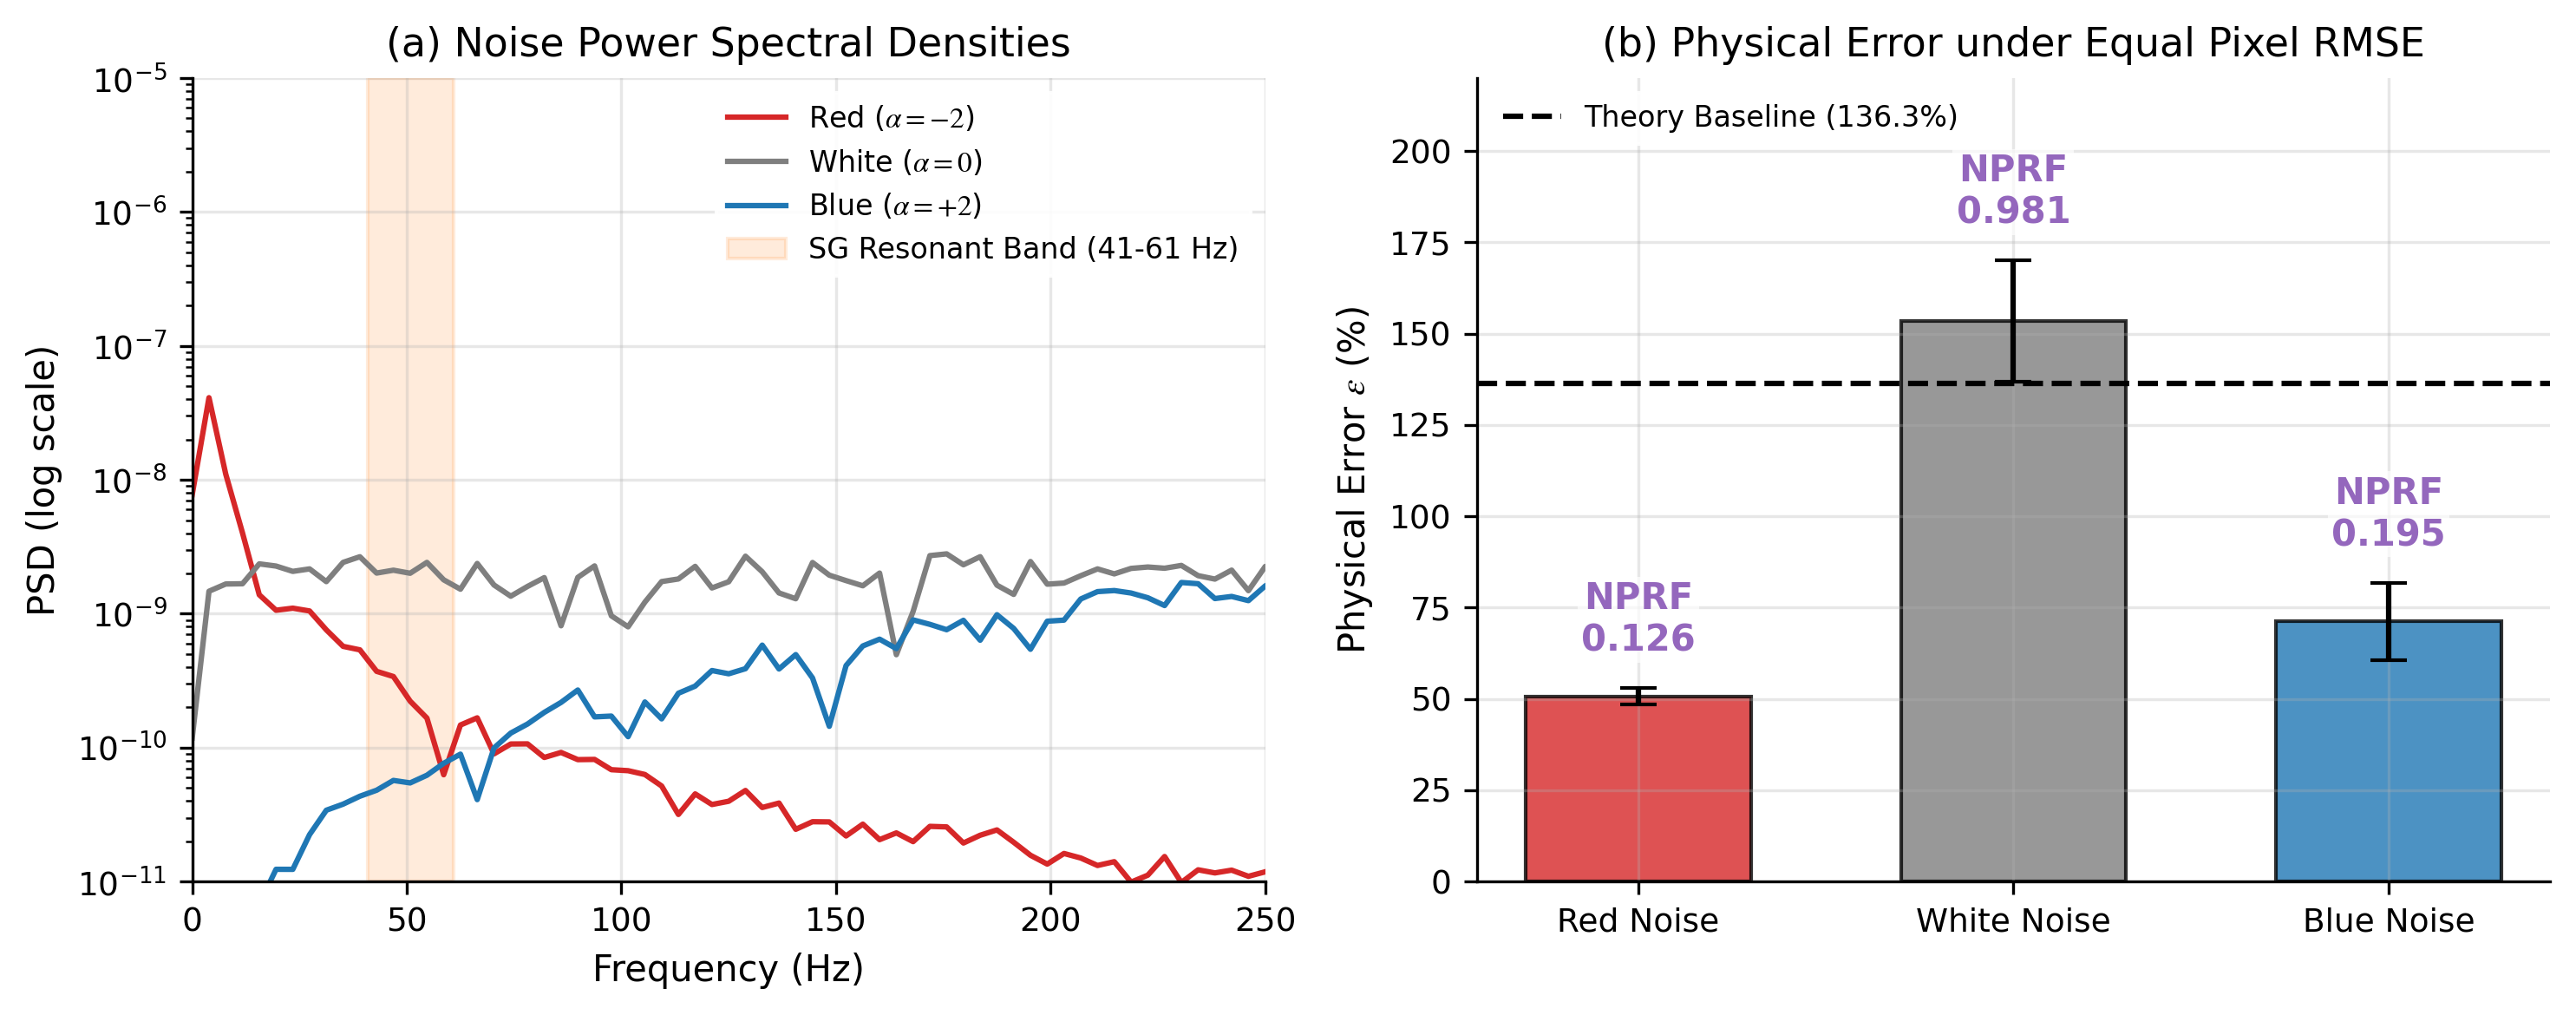
\includegraphics[width=0.8\columnwidth]{1.png}
    \caption{频谱对抗脆弱性。(a) 红/白/蓝噪声PSD；SG共振带阴影标注。(b) 相同像素RMSE下，物理误差相差3.03$\times$；NPRF正确排序风险。}
    \label{fig:fig1}
\end{figure}

\subsection{实验2：互补诊断}

\textbf{幅度主导区}（$\sigma_{\text{px}} \in [0.0005, 0.005]$，$\alpha \in [-2, 2]$，$n=500$）：像素RMSE随频谱形状一起变化。\textbf{幅度盲区}（$\sigma_{\text{px}} = 0.001$固定，$\alpha \in [-2.5, 2.5]$，$n=300$）：仅频谱形状变化。

\begin{center}
    \scriptsize\setlength{\tabcolsep}{3.5pt}
    \begin{tabular}{lcc}
        \toprule
        \textbf{区域} & \textbf{指标} & \textbf{Spearman $\bm{\rho}$} \\
        \midrule
        \multirow{2}{*}{幅度主导（$n{=}500$）} & $\pxrmse$ & $\mathbf{0.813}$ ($p<0.001$) \\
         & $\nprf$ & $0.463$ ($p<0.001$) \\
        \midrule
        \multirow{2}{*}{幅度盲区（$n{=}300$）} & $\pxrmse$ & N/A（保持恒定） \\
         & $\nprf$ & $\mathbf{0.968}$ ($p<0.001$) \\
        \bottomrule
    \end{tabular}
    \\[0.5pt]
    {\scriptsize \textbf{表2：}RMSE在幅度主导区表现最佳（$\rho=0.813$）；NPRF在幅度盲区独立接管（$\rho=0.968$）。两者缺一不可。}
\end{center}

\begin{figure}[htbp]
    \centering
    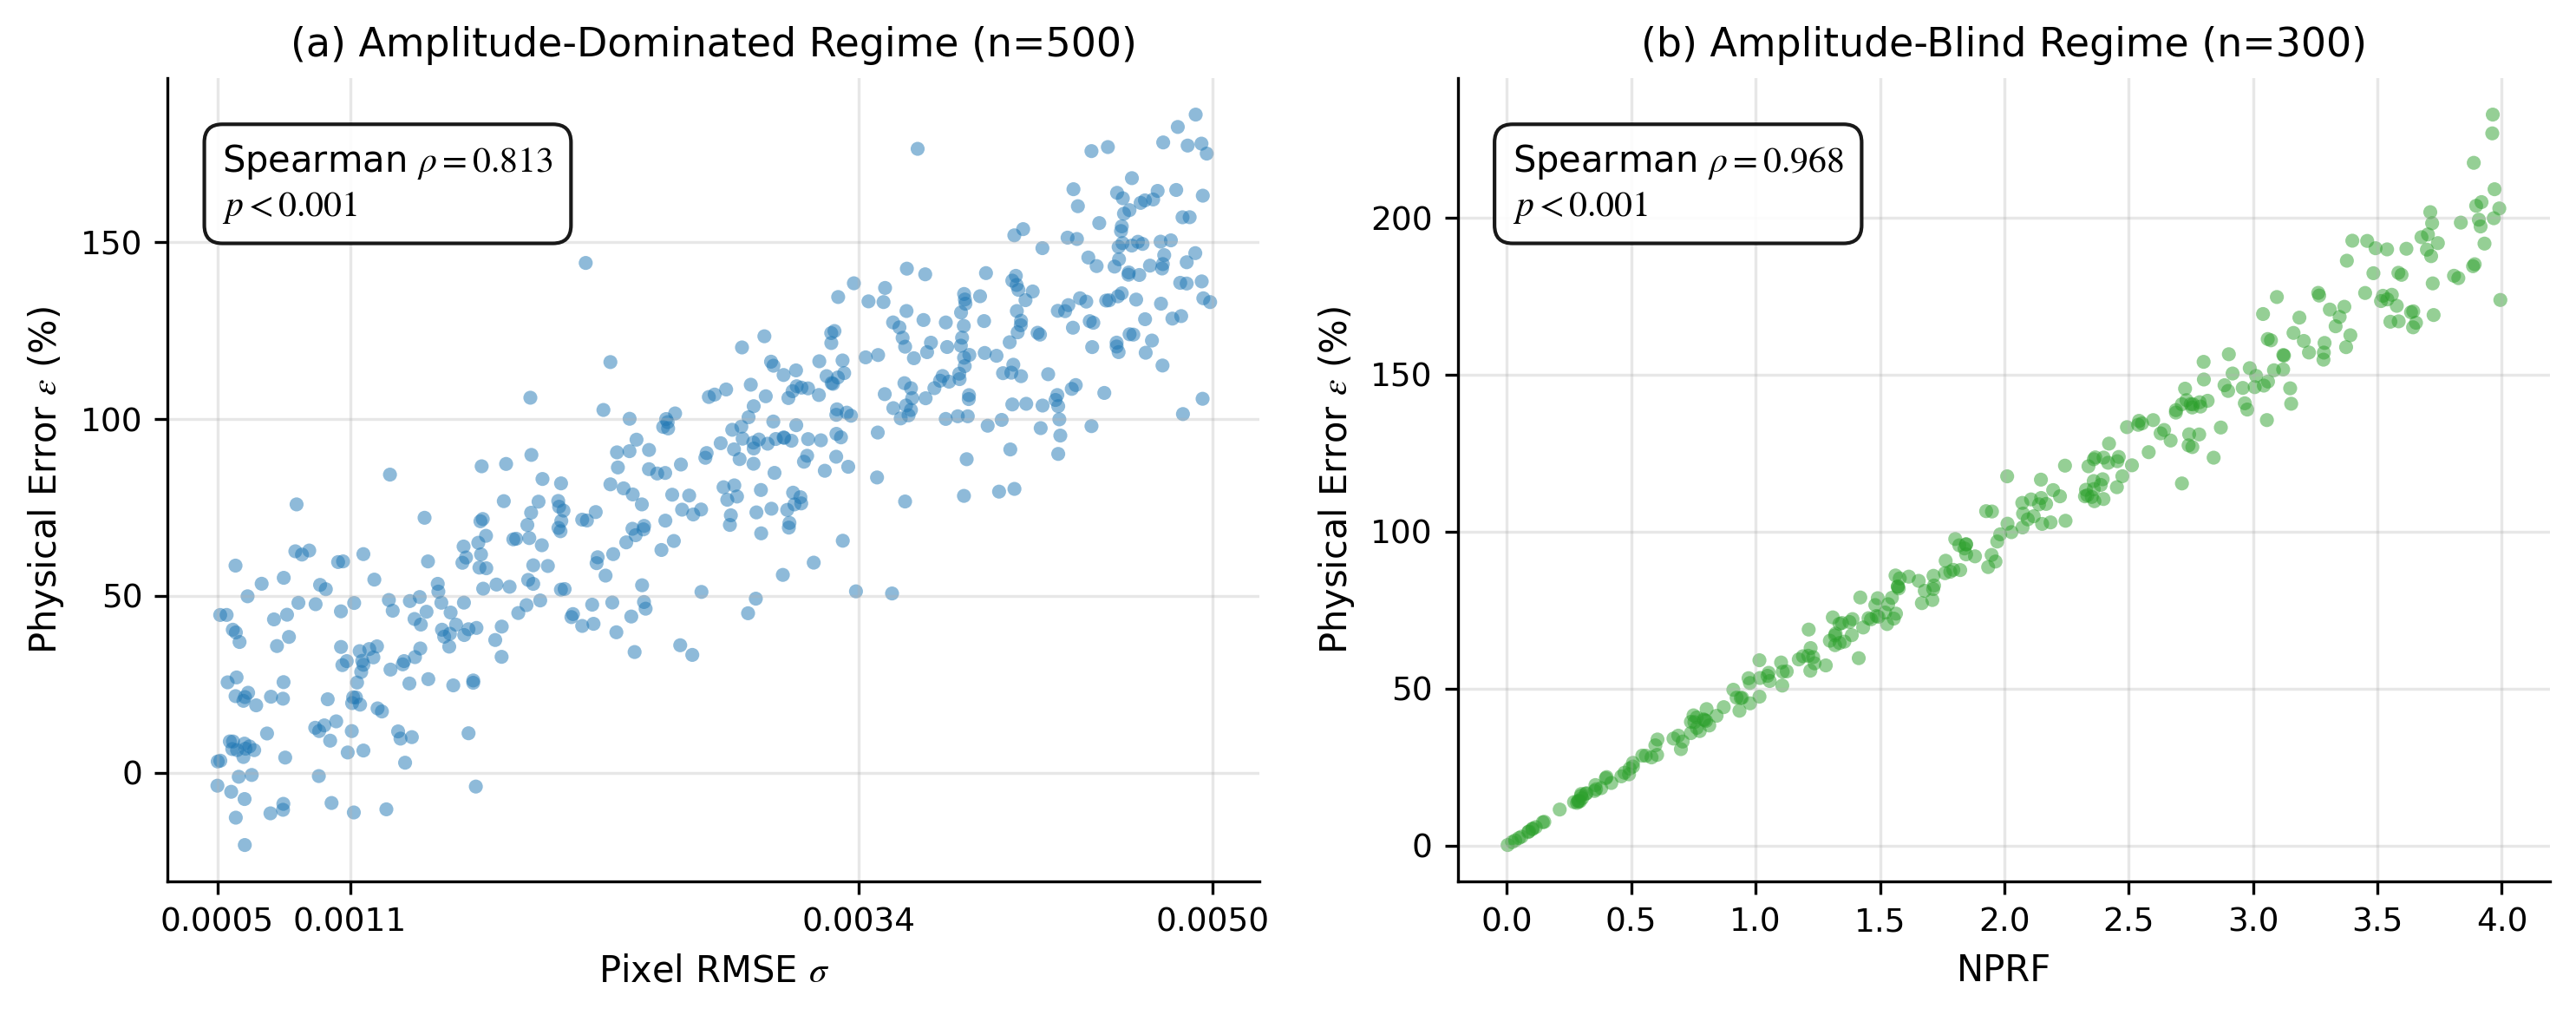
\includegraphics[width=0.8\columnwidth]{2.png}
    \caption{互补诊断。(a) 幅度主导区：RMSE强相关（$\rho=0.813$）。(b) 幅度盲区：NPRF独立排序物理误差（$\rho=0.968$）。}
    \label{fig:fig2}
\end{figure}

\subsection{实验2b：NPRF早期预警案例}

两个去噪模型具有\textit{完全相同的}像素RMSE（$\sigma_{\text{px}} = 0.00200$）：模型A（低频残差，$\alpha=-2$）；模型B（共振带残差，55--65 Hz带通）。

\begin{center}
    \scriptsize\setlength{\tabcolsep}{3.5pt}
    \begin{tabular}{lccc}
        \toprule
        \textbf{模型} & $\bm{\sigma_{\text{px}}}$ & \textbf{NPRF} & $\bm{\physerr}$(\%) \\
        \midrule
        A（低频残差） & 0.00200 & 0.113 & 98.7 \\
        B（共振残差） & 0.00200 & $\mathbf{8.875}$ & $\mathbf{815.3}$ \\
        \bottomrule
    \end{tabular}
    \\[0.5pt]
    {\scriptsize \textbf{表3：}像素RMSE相同；物理误差相差8.26$\times$；NPRF正确将模型B标记为高风险。}
\end{center}

\textbf{核心发现：}仅监控像素RMSE的从业者会认为两个模型等价；NPRF揭示了8.26$\times$的隐藏差异。

\subsection{实验3：MSE训练频谱局限性}

\textbf{设置：}干净信号10 Hz + 60 Hz（幅值1.0）。MLP去噪器（64-32，ReLU，Adam，200 epochs），$n=20$/条件。测试噪声：白+蓝，$\sigma=0.002$。\textbf{消融：}两组均用白噪声训练；组A仅使用10 Hz信号，组B使用10 Hz + 60 Hz。

\begin{center}
    \scriptsize\setlength{\tabcolsep}{2.5pt}
    \begin{tabular}{lccc}
        \toprule
        \textbf{训练噪声} & $\bm{\pxrmse}$ & $\nprf$ & $\bm{\physerr}$(\%) \\
        \midrule
        红噪声 & $0.00209_{\pm0.00039}$ & $3.701_{\pm1.767}$ & $510.5_{\pm194.0}$ \\
        白噪声 & $0.00220_{\pm0.00146}$ & $2.479_{\pm1.046}$ & $429.3_{\pm267.1}$ \\
        蓝噪声 & $0.00196_{\pm0.00052}$ & $2.590_{\pm1.273}$ & $394.7_{\pm147.7}$ \\
        \midrule
        零预测器 & $1.001$ & $5.731$ & $281219$ \\
        \bottomrule
    \end{tabular}
    \\[0.5pt]
    {\scriptsize \textbf{表4：}Kruskal-Wallis：$H=5.775$，$p=0.056$。Bonferroni校正后（$\alpha=0.0167$）\textbf{均不显著}。事后功效$\approx0.35$；\textbf{边际方向性证据}；需$n\geq60$/组。消融（仅10 Hz vs.\ 10+60 Hz）：NPRF $1.167\to2.479$，2.12倍（$p=0.000042$，Cohen's $d=1.558$）。信号型盲区是主导因果因素。}
\end{center}

\textbf{核心发现：}\textbf{第一，}模型学会了去噪（$\pxrmse$下降约500倍）。\textbf{第二，}训练噪声效应在校正后\textit{不}具有统计显著性。\textbf{第三，}所有模型NPRF$>1.0$——双重盲区：噪声型（蓝训练：2.590 vs.\ 基线0.195）和信号型（60 Hz位于共振带内）。仅靠MSE训练本身不能带来频谱免疫能力；必须通过外部手段引入。

\begin{figure}[htbp]
    \centering
    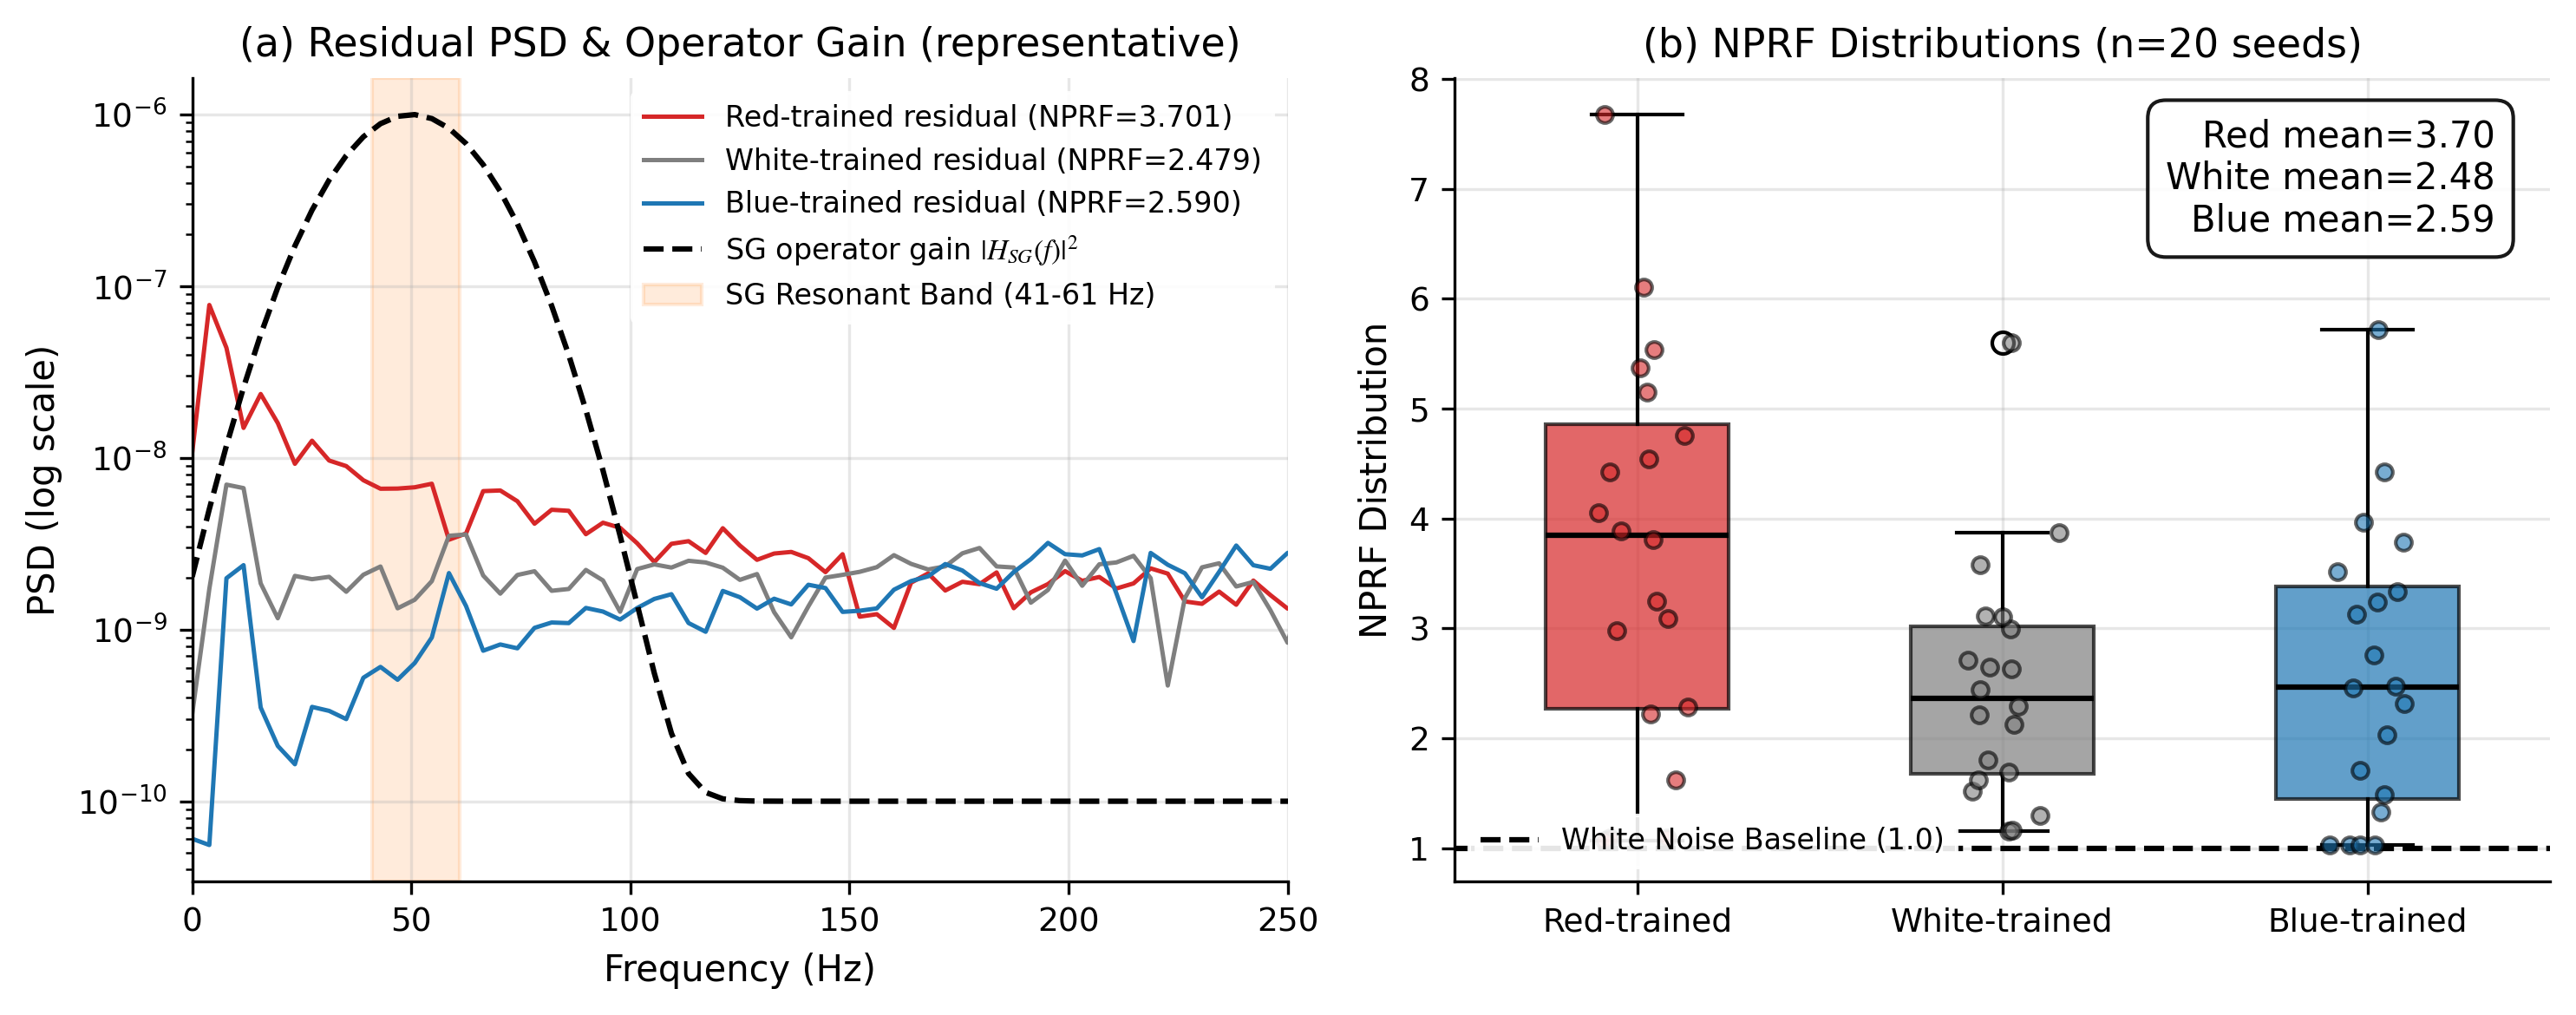
\includegraphics[width=0.8\columnwidth]{3.png}
    \caption{标准MSE训练的频谱盲区。(a) 残差PSD（seed-0）；红训练模型留下共振带能量。(b) NPRF分布（$n=20$）；全部超过基线1.0。}
    \label{fig:fig3}
\end{figure}

\subsection{实验3b：后处理频谱重塑作为补救}

训练时频谱正则化被证明数值不稳定（NPRF是比率指标，其梯度在$\sigma_{\text{px}}\to0$时发散；共振带惩罚与60 Hz信号保留冲突）。我们采用\textbf{后处理频谱重塑}：在标准MSE残差上应用五级IIR陷波（45/48/51/54/57 Hz，$Q=8.0$）。

\begin{center}
    \scriptsize\setlength{\tabcolsep}{3.5pt}
    \begin{tabular}{lccc}
        \toprule
        \textbf{阶段} & \textbf{NPRF} & $\bm{\physerr}$(\%) & $\bm{\sigma_{\text{px}}}$ \\
        \midrule
        重塑前 & $2.412_{\pm0.797}$ & $348.2_{\pm114.9}$ & $0.00174_{\pm0.00035}$ \\
        重塑后 & $\mathbf{1.210_{\pm0.312}}$ & $\mathbf{240.4_{\pm74.9}}$ & $0.00160_{\pm0.00028}$ \\
        \bottomrule
    \end{tabular}
    \\[0.5pt]
    {\scriptsize \textbf{表5：}后处理陷波滤波将NPRF降低49.8\%，物理误差降低31.0\%（$p=0.001953$，$n=10$配对）。像素RMSE基本不变（$-8.0\%$）。}
\end{center}

\textbf{关键：}无需重新训练的频谱免疫——即插即用陷波滤波器重塑残差频谱。像素RMSE代价可忽略（$<10\%$），因为陷波仅移除$4\%$带宽。

\subsection{实验4：频域解剖}

围绕共振峰$f_{\text{peak}}=51$ Hz的频段：亚共振（0--41 Hz）、共振（41--61 Hz）、抑制（61--500 Hz）。

\begin{center}
    \scriptsize
    \resizebox{\columnwidth}{!}{%
    \begin{tabular}{lccccc}
        \toprule
        \textbf{频段} & \textbf{带宽占比(\%)} & \textbf{白贡献(\%)} & \textbf{蓝贡献(\%)} & \textbf{效率比} \\
        \midrule
        亚共振 & 8.2 & 15.2 & 0.8 & 1.86 \\
        共振 & 4.0 & \textbf{42.8} & 5.9 & \textbf{10.70} \\
        抑制 & 87.8 & 42.0 & \textbf{93.3} & 0.48 \\
        \bottomrule
    \end{tabular}%
    }
    \\[0.5pt]
    {\scriptsize \textbf{表6：}效率比 = 贡献(\%) / 带宽占比(\%)，衡量单位带宽的风险集中度。仅4.0\%带宽占比的共振带贡献了白噪声42.8\%的积分物理误差（效率比10.70）。蓝噪声能量集中在抑制带（93.3\%）。}
\end{center}

\textbf{核心发现：}共振带风险效率是全频带平均的10.70$\times$，确认频谱免疫策略应优先考虑共振带缓解。

\subsection{实验5：工程验证}

\textbf{设置：}100个非稳态噪声样本（$\alpha\in[0,2]$，$\sigma\in[0.0020,0.0035]$）。A：无滤波；B：Butterworth $f_c=150$ Hz；C：五级IIR陷波（45/48/51/54/57 Hz，$Q=8.0$）。

\begin{center}
    \scriptsize
    \resizebox{\columnwidth}{!}{%
    \begin{tabular}{lccc}
        \toprule
        \textbf{滤波器} & $\bm{\physerr}$(\%) & $\nprf$ & \textbf{像素RMSE} \\
        \midrule
        A（无处理） & $292.4_{\pm51.0}$ & $0.448_{\pm0.087}$ & $0.00277_{\pm0.00015}$ \\
        B（Butterworth） & $229.7_{\pm36.0}$ & $2.151_{\pm0.431}$ & $0.00097_{\pm0.00010}$ \\
        C（频谱免疫） & $272.3_{\pm45.8}$ & $\mathbf{0.440_{\pm0.094}}$ & $0.00260_{\pm0.00014}$ \\
        \bottomrule
    \end{tabular}%
    }
    \\[0.5pt]
    {\scriptsize \textbf{表7：}Mann-Whitney U：A vs B $p<0.001$；A vs C $p=0.0011$。Butterworth将NPRF推高+380.0\%：$f_c=150$ Hz对带外能量的抑制远大于共振带能量，导致$\sigma_{\text{px}}^2$（分母）下降快于加权分子。陷波器维持NPRF接近基线。比值法预测偏差：2.4\%。}
\end{center}

\begin{figure}[htbp]
    \centering
    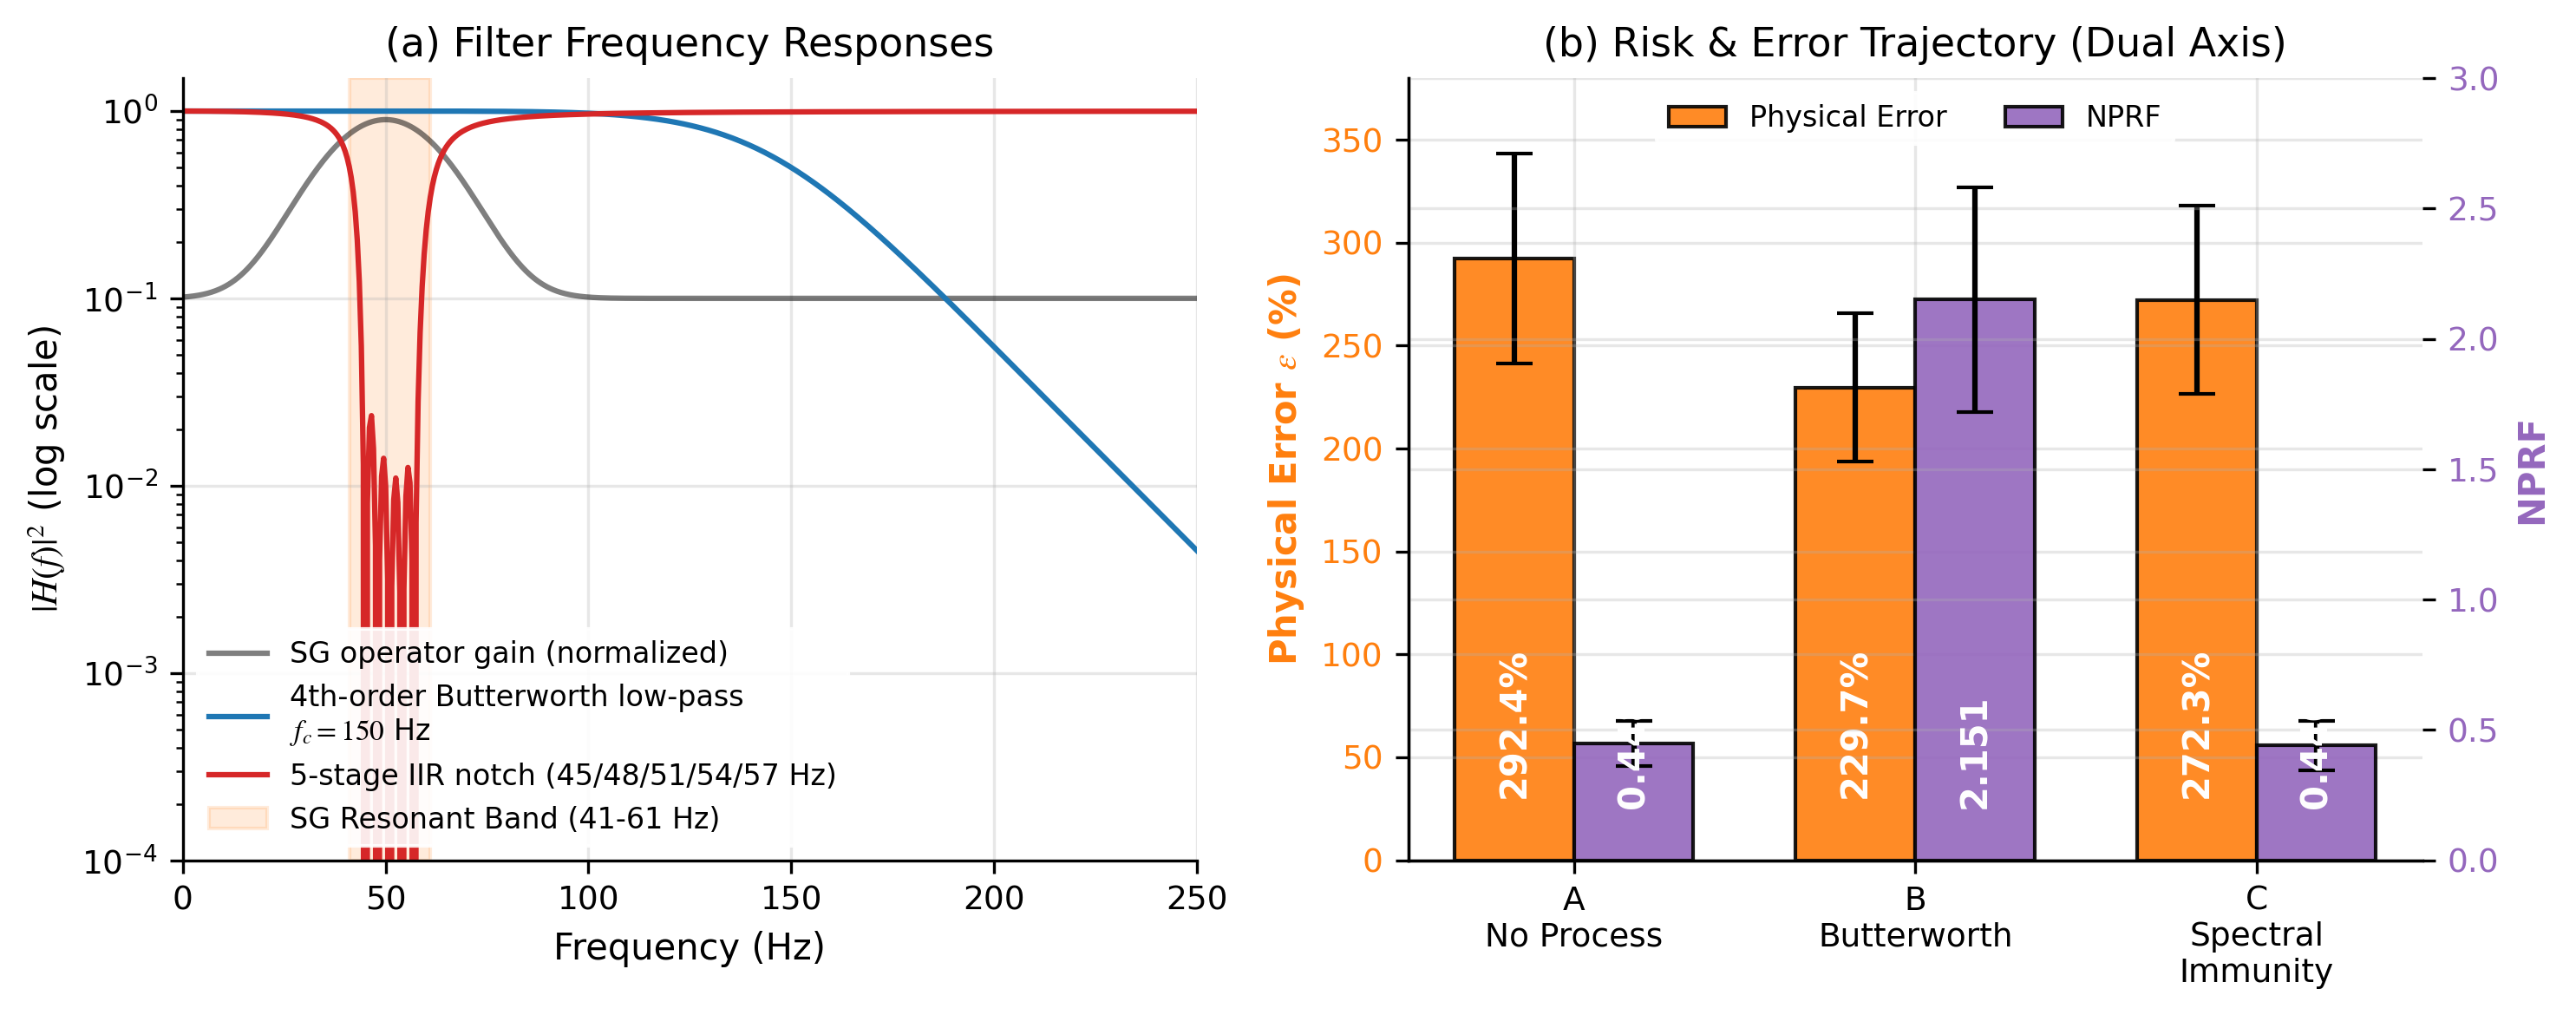
\includegraphics[width=0.8\columnwidth]{4.png}
    \caption{工程验证。(a) 滤波器响应 vs.\ SG共振带；陷波器衰减共振能量，Butterworth则不然。(b) NPRF vs.\ 物理误差（$n=100$）。}
    \label{fig:fig4}
\end{figure}

\subsection{实验6：真实世界篮球抛体（无统计声明）}

\textbf{设置：}DJI Action（48 fps），53帧手动追踪。篮球直径0.246 m $\approx$ 40 px，比例$6.15\times10^{-3}$ m/px。二维抛体：$x(t)$线性，$y(t)$二次。

\begin{center}
    \scriptsize\setlength{\tabcolsep}{3.5pt}
    \begin{tabular}{lcc}
        \toprule
        \textbf{物理量} & \textbf{数值} & \textbf{说明} \\
        \midrule
        $v_{0x}$ & 5.20 m/s & $R^2=0.9974$ \\
        $a_y$ & $-11.29$ m/s$^2$ & 相对$g$偏差15.2\% \\
        $\sigma_x$ / $\sigma_y$ & 84.9 / 67.0 mm & 追踪噪声 \\
        逐帧物理误差 & 75.3\% & SG瞬时$a$ \\
        NPRF & 0.177 & 仅概念 \\
        \bottomrule
    \end{tabular}
    \\[0.5pt]
    {\scriptsize \textbf{表8：}偏差来源：标定（$\pm5\%$）、镜头畸变、空气阻力（$g$的0.3\%）。$N=53$：无法计算置信区间；NPRF仅作为工作流演示。流程端到端执行时间$<$1 s。}
\end{center}

% ==================== 4. 局限性与部署 ====================
\section{局限性与部署}

\subsection{局限性}

\textbf{线性算子假设}对强非线性算子可能失效。\textbf{标定依赖性：}黑盒流程需要数值扰动。\textbf{统计功效：}实验3边际性（$p=0.056$，功效$\approx0.35$）；消融充分（$p=0.000042$）。\textbf{信号-噪声重叠：}陷波滤波器衰减真实60 Hz信号。\textbf{Welch泄漏：}$N<200$仅筛查。\textbf{PGTS到真实世界的差距：}定量结果仅在PGTS内。NPRF补充UQ：UQ问"有多不确定？"NPRF问"在物理上有多危险？"

\subsection{部署}

\textbf{(1) AI-for-Science的频谱健康检查：}每次预测后计算NPRF，无需昂贵的DFT验证。\textbf{(2) 视觉追踪：}NPRF$>2.0$时触发"减速"。\textbf{(3) 质量门控：}NPRF$>1.5$--$2.0$时标记低置信度，无需金标准标注\cite{ardila2019}。

\subsection{未来工作}

频谱对抗训练（共振带能量惩罚，平方范数，避免比率梯度不稳定）。自适应陷波滤波器。非线性扩展（Volterra级数）。NPRF渐近理论。真实场景验证。理想矩形陷波上界用于频谱免疫滤波器基准测试。

% ==================== 5. 结论 ====================
\section{结论}

像素RMSE在物理量导出流程中存在结构性失效：相同像素误差幅值可产生3.03$\times$（一般情况）至8.26$\times$（对抗情况）的物理误差差异。本文提出首个频谱理论解，将信任从"像素基础"转向"频谱基础"。

核心贡献：（1）频谱充分性定理（定理\ref{thm:sufficiency}）；（2）无需物理真值的NPRF（式\ref{eq:nprf_def}）；（3）RMSE+NPRF双范式；（4）早期预警（8.26$\times$差异）；（5）后处理补救（NPRF $-49.8\%$，$p=0.002$）；（6）反直觉Butterworth发现（+380.0\% NPRF）；（7）MSE双重盲区与消融（$p=0.000042$，$d=1.558$）；（8）真实世界概念验证。

\begingroup
\scriptsize
\textbf{边界声明：}已证明：（1）算子共振下像素RMSE的结构性失效；（2）NPRF可行性；（3）MSE频谱盲区；（4）PGTS内后处理重塑有效性。\textbf{未}证明：（a）NPRF对任意非线性算子的有效性；（b）滤波器在PGTS之外的泛化性；（c）训练噪声类型显著性（$p=0.056$，功效$\approx0.35$）。
\endgroup

\vspace{1pt}

每个从观测数据导出物理量的AI科学家，无论是否知情，都在对其残差误差的频谱平坦性下注。本文表明这一赌注经常失败。\textbf{频谱疫苗}——NPRF诊断加后处理频谱免疫滤波——提供了首个可部署的免疫应答。NPRF的即插即用特性——无需真值、最小开销、离线标定——使其成为基础设施的候选组件。\textbf{未来的AI科学家不仅需要强大的推理能力，还需要一套内生的免疫系统——在每次输出之前自主询问：我的结果在物理上可信吗？}

\vspace{1pt}
{\scriptsize\noindent\textbf{致谢：}感谢指导教师滕伟老师、班主任张明璐老师、牛政老师及年级主任任倩老师的支持与帮助。
\vspace{1pt}
{\scriptsize\noindent\textbf{作者贡献：}杨御之与\name 对本文贡献均等。杨御之提出问题、构建理论框架并设计实验；\name 完成频域分析、实现全部代码并执行数值实验。两位作者共同分析结果并撰写论文。}
代码：\texttt{https://github.com/RosslynKira/spectral-immunity}}

% ==================== 参考文献 ====================
\begingroup
\scriptsize
\setlength{\itemsep}{0.5pt}
\setlength{\parsep}{0pt}
\renewcommand{\baselinestretch}{0.72}
\begin{thebibliography}{99}

\bibitem{abramson2024}
J.~Abramson, J.~Adler, J.~Dunger, et al.
\newblock Accurate structure prediction of biomolecular interactions with AlphaFold 3.
\newblock \textit{Nature}, 630:493--500, 2024.

\bibitem{merchant2023}
A.~Merchant, S.~Batzner, S.~S.~Schoenholz, et al.
\newblock Scaling deep learning for materials discovery.
\newblock \textit{Nature}, 624:80--85, 2023.

\bibitem{lam2023}
R.~Lam, A.~Sanchez-Gonzalez, M.~Willson, et al.
\newblock Learning skillful medium-range global weather forecasting.
\newblock \textit{Science}, 382:1416--1421, 2023.

\bibitem{savitzky1964}
A.~Savitzky and M.~J.~E.~Golay.
\newblock Smoothing and differentiation of data by simplified least squares procedures.
\newblock \textit{Analytical Chemistry}, 36(8):1627--1639, 1964.

\bibitem{welch1967}
P.~D.~Welch.
\newblock The use of fast Fourier transform for the estimation of power spectra: a method based on time averaging over short, modified periodograms.
\newblock \textit{IEEE Transactions on Audio and Electroacoustics}, 15(2):70--73, 1967.

\bibitem{brillinger2001}
D.~R.~Brillinger.
\newblock \textit{Time Series: Data Analysis and Theory}. SIAM, 2001.

\bibitem{kasdin1995}
N.~J.~Kasdin.
\newblock Discrete simulation of colored noise and stochastic processes and $1/f^\alpha$ power law noise generation.
\newblock \textit{Proceedings of the IEEE}, 83(5):802--827, 1995.

\bibitem{burger2020}
B.~Burger, P.~M.~Maffettone, V.~V.~Gusev, et al.
\newblock A mobile robotic chemist.
\newblock \textit{Nature}, 583:237--241, 2020.

\bibitem{xu2019}
Z.-Q.~J.~Xu, Y.~Zhang, and Y.~Xiao.
\newblock Training behavior of deep neural network in frequency domain.
\newblock In \textit{Neural Information Processing, ICONIP 2019}, LNCS 11953, pp.~264--274, Springer, 2019.

\bibitem{ardila2019}
D.~Ardila, A.~P.~Kiraly, S.~Bharadwaj, et al.
\newblock End-to-end lung cancer screening with three-dimensional deep learning on low-dose chest computed tomography.
\newblock \textit{Nature Medicine}, 25(6):954--961, 2019.

\bibitem{rahaman2019}
N.~Rahaman, A.~Baratin, D.~Arpit, et al.
\newblock On the spectral bias of neural networks.
\newblock \textit{Proceedings of the 36th International Conference on Machine Learning}, PMLR 97:5301--5310, 2019.

\bibitem{kendall2017}
A.~Kendall and Y.~Gal.
\newblock What uncertainties do we need in Bayesian deep learning for computer vision?
\newblock \textit{Advances in Neural Information Processing Systems 30}, 2017.

\bibitem{lakshminarayanan2017}
B.~Lakshminarayanan, A.~Pritzel, and C.~Blundell.
\newblock Simple and scalable predictive uncertainty estimation using deep ensembles.
\newblock \textit{Advances in Neural Information Processing Systems 30}, 2017.

\bibitem{tancik2020}
M.~Tancik, P.~P.~Srinivasan, B.~Mildenhall, et al.
\newblock Fourier features let networks learn high frequency functions in low dimensional domains.
\newblock \textit{Advances in Neural Information Processing Systems 33}, 2020.

\bibitem{ronen2019}
R.~Basri, D.~Jacobs, Y.~Kasten, and S.~Kritchman.
\newblock The convergence rate of neural networks for learned functions of different frequencies.
\newblock \textit{Advances in Neural Information Processing Systems 32}, pp.~4761--4771, 2019.

\end{thebibliography}
\endgroup

\end{document}